\documentclass[11pt]{article}
\usepackage[textwidth=18.0cm, textheight=23.0cm, top=2.0cm]{geometry}
\usepackage{pst-all}
\usepackage{amssymb}
\usepackage{tikz}
\usepackage{underscore}\begin{document}
\pagestyle{empty}


ClassName: \underline{\textbf{Class_07.2bp-15}}
\par
BinSize: \underline{\textbf{100 × 100}}
\par
ReduceSize: \underline{\textbf{100 × 100}}
\par
TypeNum: \underline{\textbf{40}}
\par
Num: \underline{\textbf{40}}
\par
OutS: \underline{\textbf{110000}}
\par
InS: \underline{\textbf{95584}}
\par
Rate: \underline{\textbf{0.869}}
\par
UB: \underline{\textbf{11}}
\par
LB0: \underline{\textbf{11}}
\par
LB: \underline{\textbf{11}}
\par
LBWithCut: \underline{\textbf{11}}
\par
NodeCut: \underline{\textbf{0}}
\par
ExtendedNodeCnt: \underline{\textbf{1}}
\par
GenNodeCnt: \underline{\textbf{1}}
\par
PrimalNode: \underline{\textbf{0}}
\par
ColumnCount: \underline{\textbf{11}}
\par
TotalCutCount: \underline{\textbf{0}}
\par
RootCutCount: \underline{\textbf{0}}
\par
LPSolverCnt: \underline{\textbf{1}}
\par
PricingSolverCnt: \underline{\textbf{0}}
\par
BranchAndBoundNum: \underline{\textbf{1}}
\par
isOpt: \underline{\textbf{true}}
\par
TimeOnInitSolution: \underline{\textbf{0.120 s}}
\par
TimeOnPrimal: \underline{\textbf{0.000 s}}
\par
TimeOnPricing: \underline{\textbf{0.000 s}}
\par
TimeOnRmp: \underline{\textbf{0.063 s}}
\par
TotalTime: \underline{\textbf{0.230 s}}
\par
\newpage


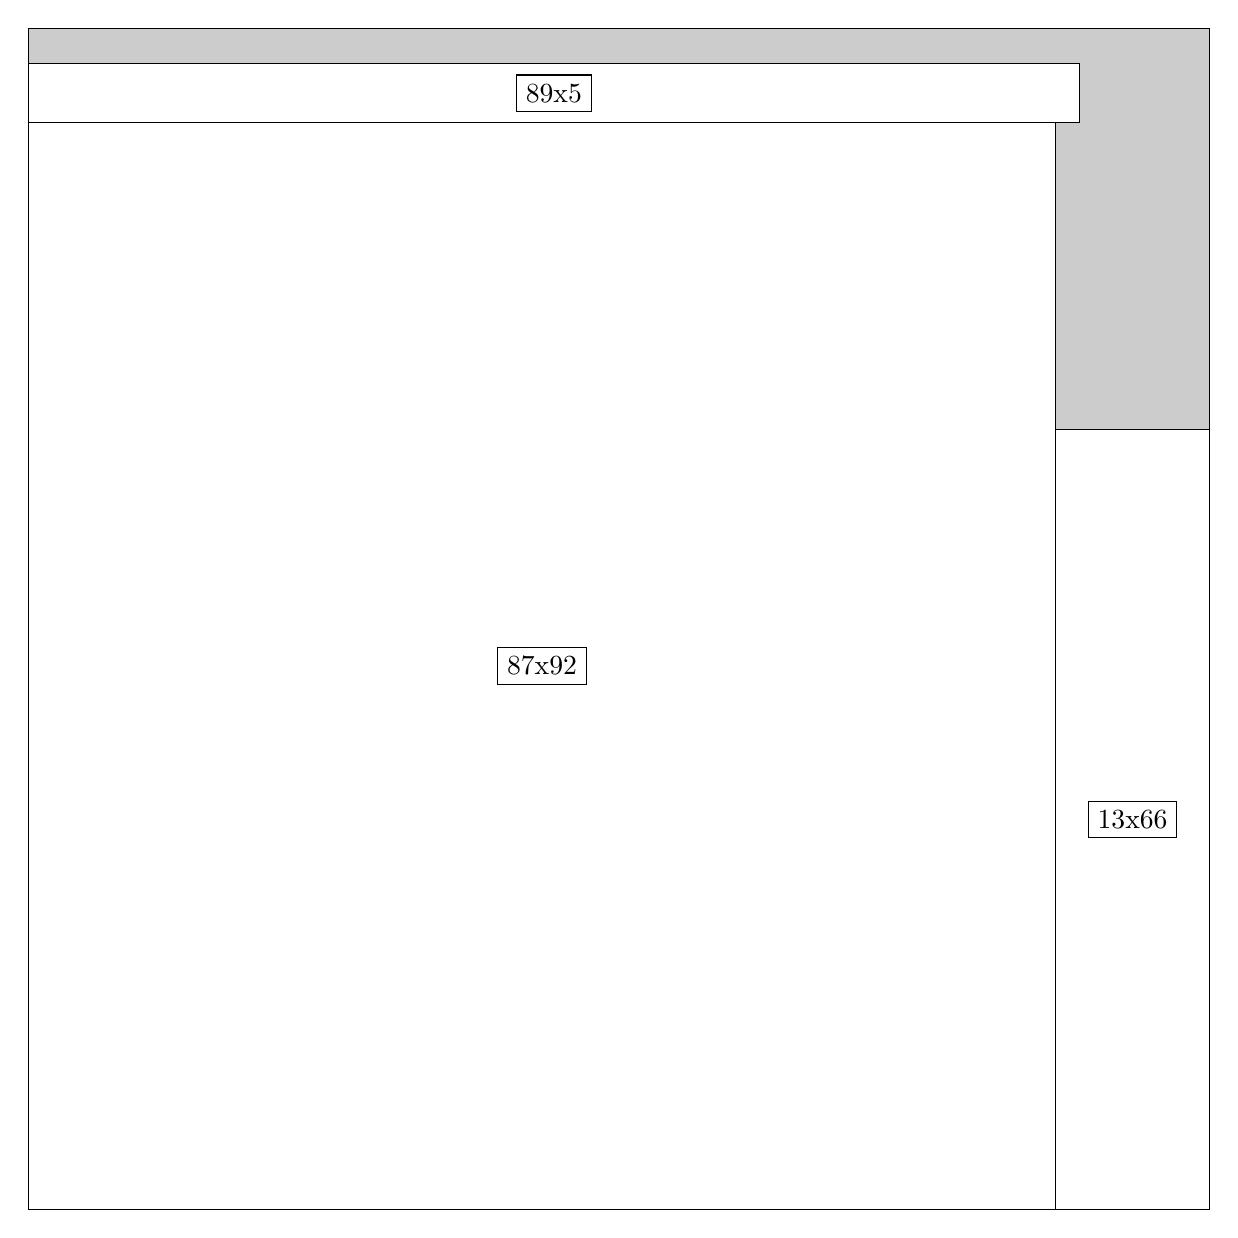
\begin{tikzpicture}[shorten >=1pt,scale=1.0,every node/.style={scale=1.0},->]
\tikzstyle{vertex}=[circle,fill=black!25,minimum size=14pt,inner sep=0pt]
\filldraw[fill=gray!40!white, draw=black] (0,0) rectangle (15.0,15.0);
\foreach \name/\x/\y/\w/\h in {87x92/0.0/0.0/13.049999999999999/13.799999999999999,13x66/13.049999999999999/0.0/1.95/9.9,89x5/0.0/13.799999999999999/13.35/0.75}
\filldraw[fill=white!40!white, draw=black] (\x,\y) rectangle node[draw] (\name) {\name} ++(\w,\h);
\end{tikzpicture}


w =87 , h =92 , x =0 , y =0 , v =8004
\par
w =13 , h =66 , x =87 , y =0 , v =858
\par
w =89 , h =5 , x =0 , y =92 , v =445
\par
\newpage


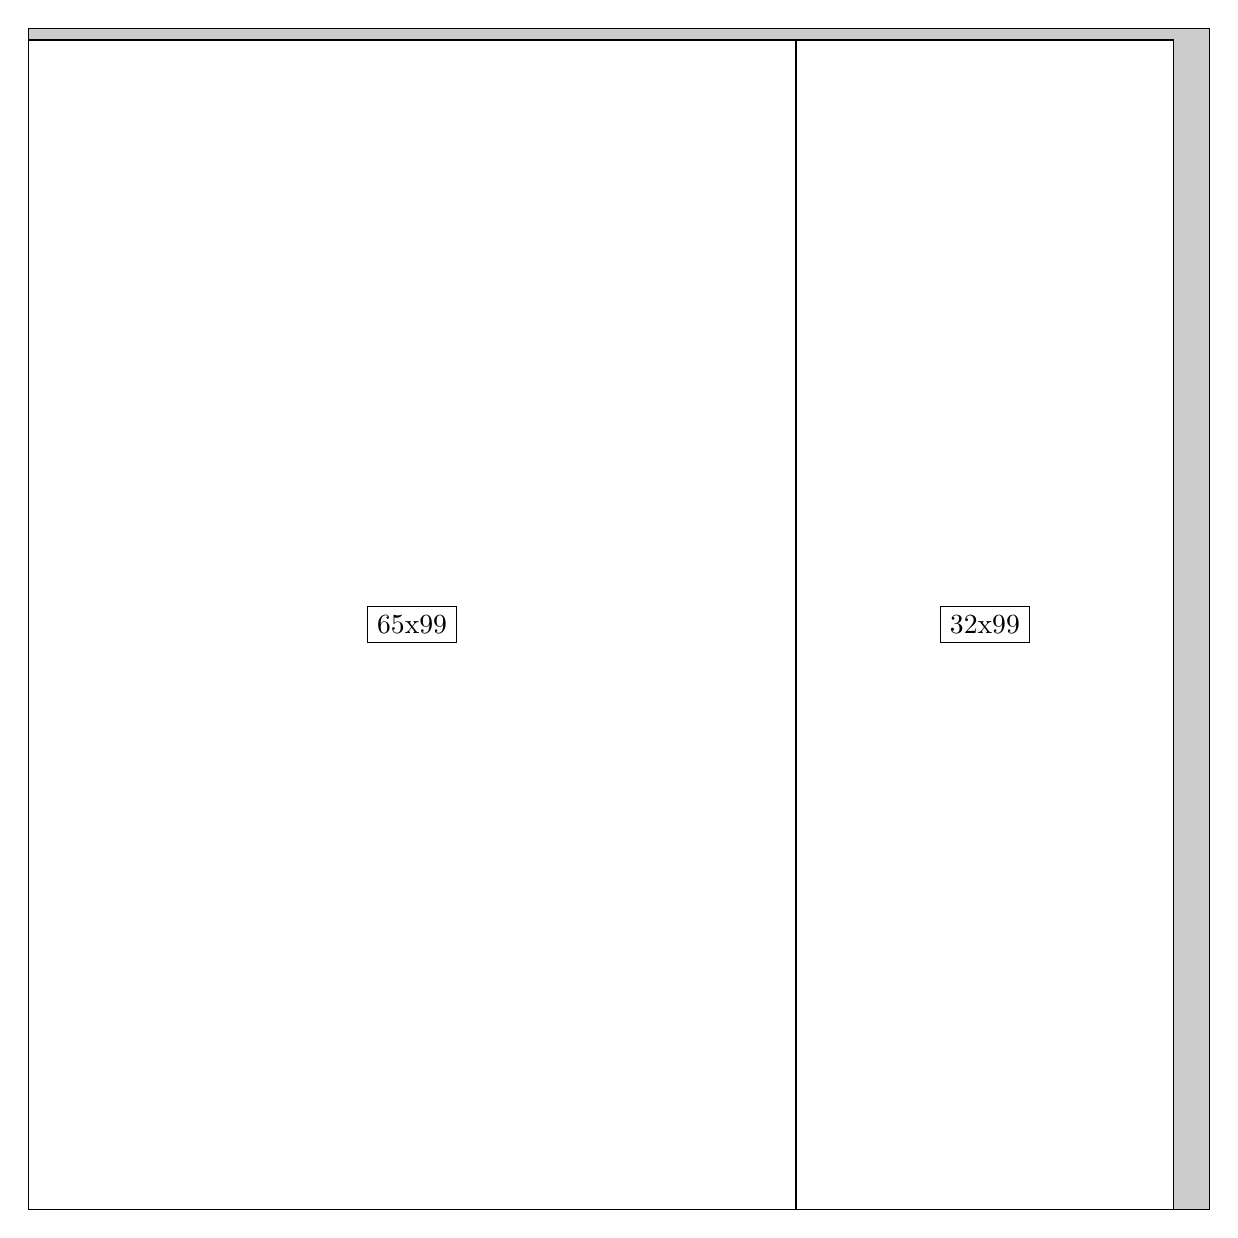
\begin{tikzpicture}[shorten >=1pt,scale=1.0,every node/.style={scale=1.0},->]
\tikzstyle{vertex}=[circle,fill=black!25,minimum size=14pt,inner sep=0pt]
\filldraw[fill=gray!40!white, draw=black] (0,0) rectangle (15.0,15.0);
\foreach \name/\x/\y/\w/\h in {65x99/0.0/0.0/9.75/14.85,32x99/9.75/0.0/4.8/14.85}
\filldraw[fill=white!40!white, draw=black] (\x,\y) rectangle node[draw] (\name) {\name} ++(\w,\h);
\end{tikzpicture}


w =65 , h =99 , x =0 , y =0 , v =6435
\par
w =32 , h =99 , x =65 , y =0 , v =3168
\par
\newpage


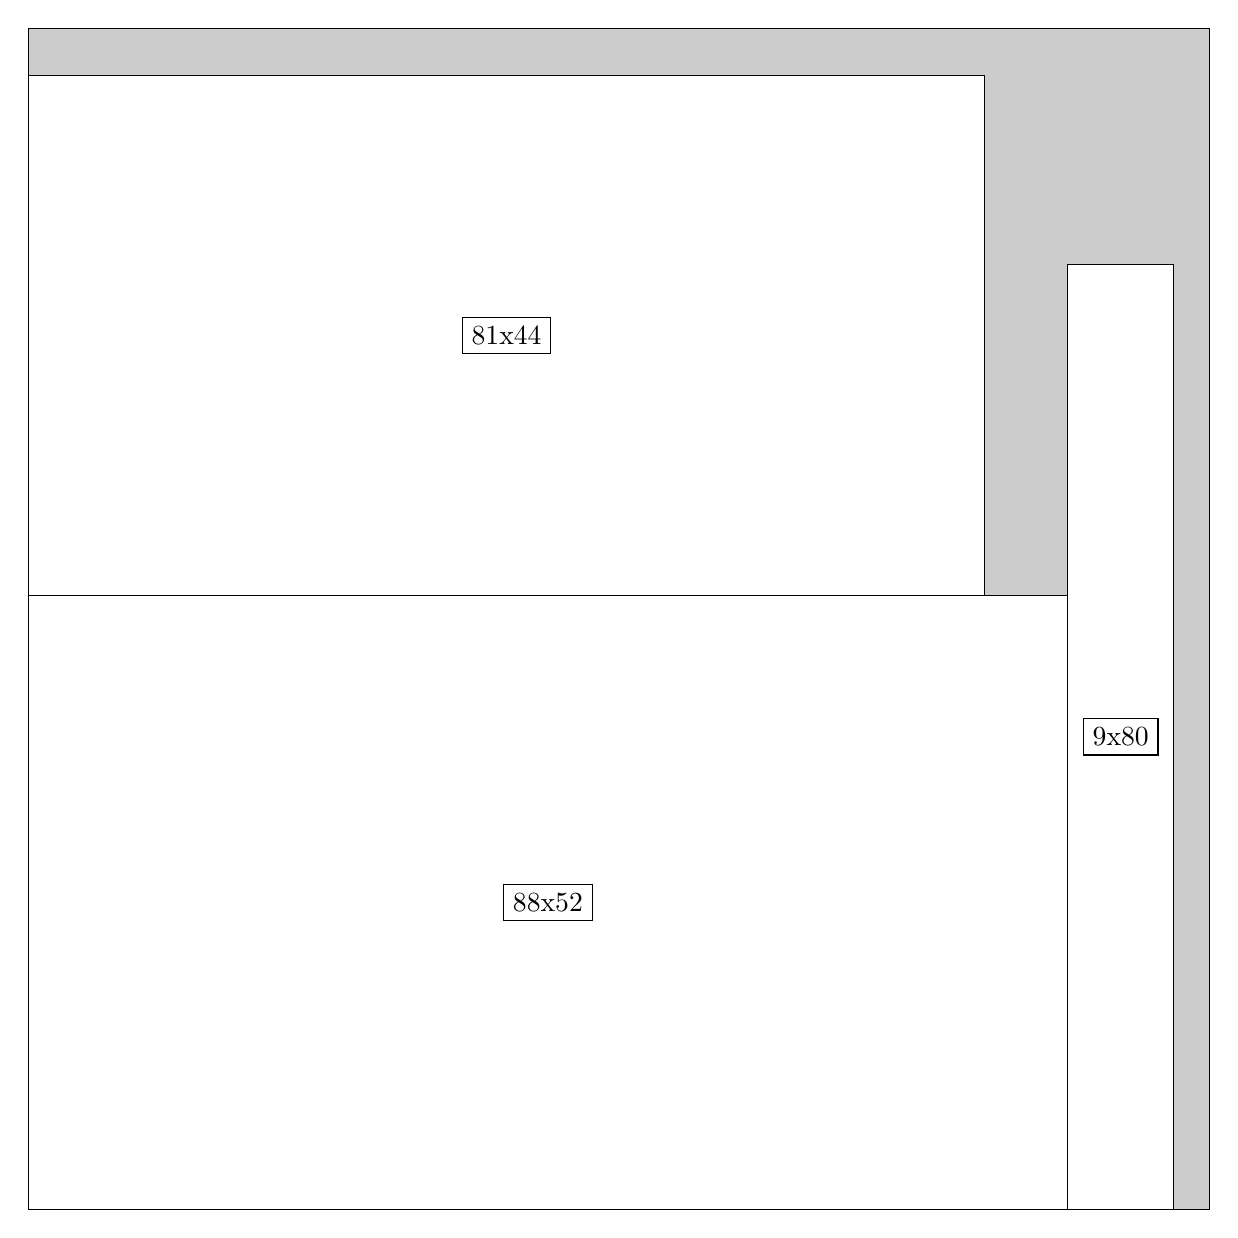
\begin{tikzpicture}[shorten >=1pt,scale=1.0,every node/.style={scale=1.0},->]
\tikzstyle{vertex}=[circle,fill=black!25,minimum size=14pt,inner sep=0pt]
\filldraw[fill=gray!40!white, draw=black] (0,0) rectangle (15.0,15.0);
\foreach \name/\x/\y/\w/\h in {81x44/0.0/7.8/12.15/6.6,88x52/0.0/0.0/13.2/7.8,9x80/13.2/0.0/1.3499999999999999/12.0}
\filldraw[fill=white!40!white, draw=black] (\x,\y) rectangle node[draw] (\name) {\name} ++(\w,\h);
\end{tikzpicture}


w =81 , h =44 , x =0 , y =52 , v =3564
\par
w =88 , h =52 , x =0 , y =0 , v =4576
\par
w =9 , h =80 , x =88 , y =0 , v =720
\par
\newpage


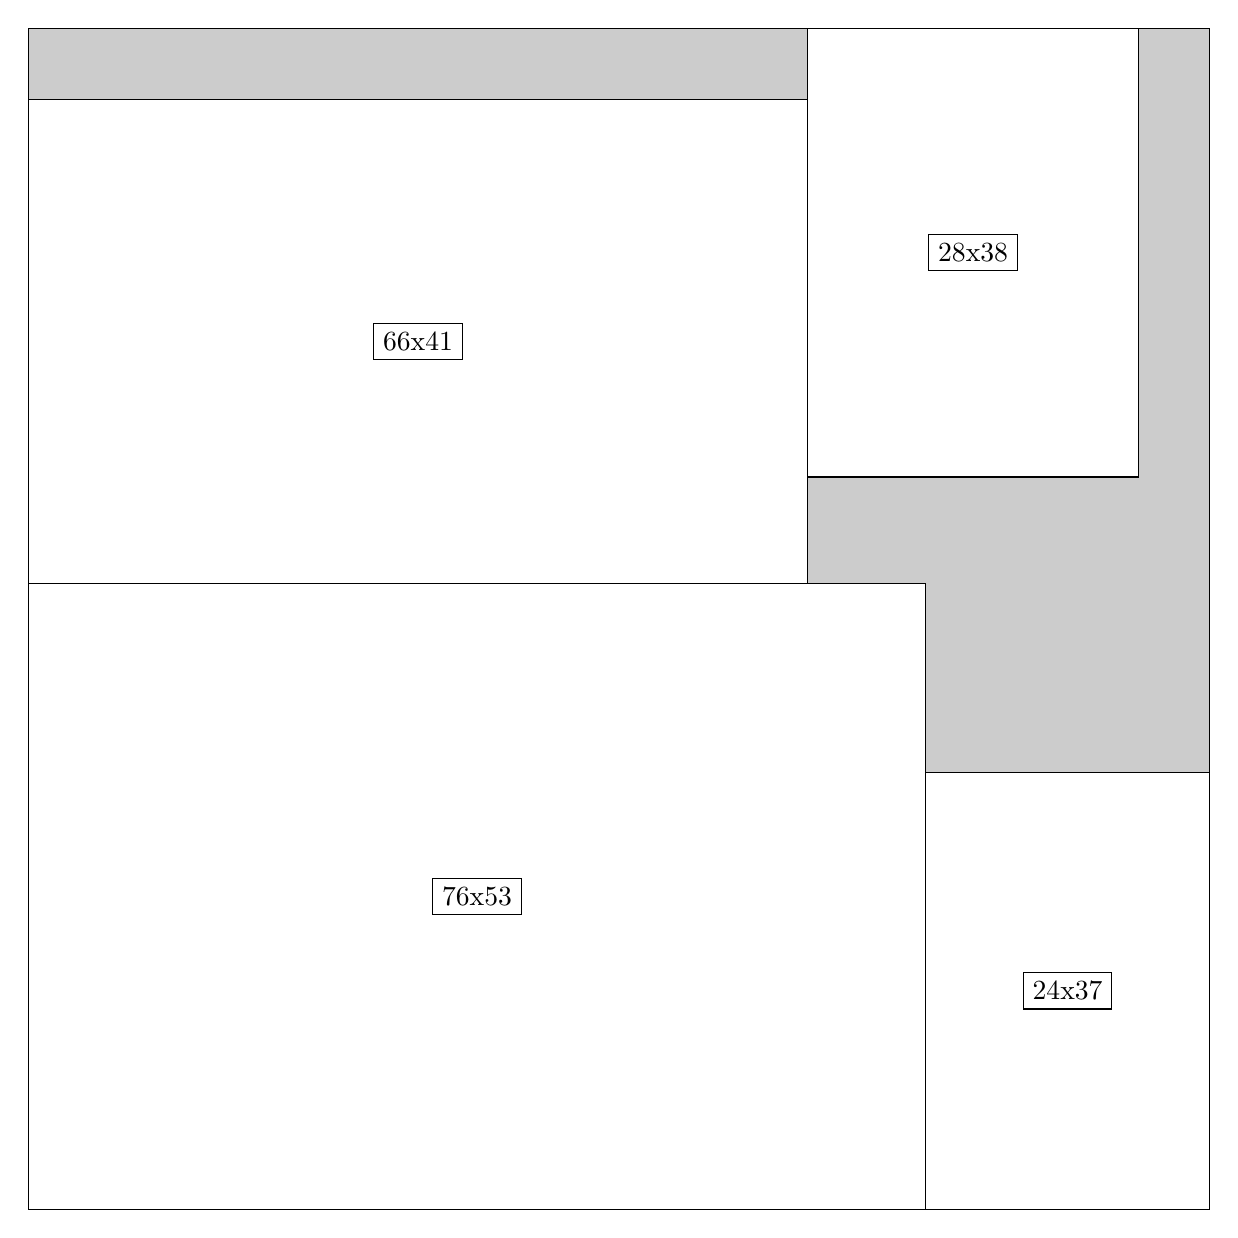
\begin{tikzpicture}[shorten >=1pt,scale=1.0,every node/.style={scale=1.0},->]
\tikzstyle{vertex}=[circle,fill=black!25,minimum size=14pt,inner sep=0pt]
\filldraw[fill=gray!40!white, draw=black] (0,0) rectangle (15.0,15.0);
\foreach \name/\x/\y/\w/\h in {76x53/0.0/0.0/11.4/7.949999999999999,66x41/0.0/7.949999999999999/9.9/6.1499999999999995,28x38/9.9/9.299999999999999/4.2/5.7,24x37/11.4/0.0/3.5999999999999996/5.55}
\filldraw[fill=white!40!white, draw=black] (\x,\y) rectangle node[draw] (\name) {\name} ++(\w,\h);
\end{tikzpicture}


w =76 , h =53 , x =0 , y =0 , v =4028
\par
w =66 , h =41 , x =0 , y =53 , v =2706
\par
w =28 , h =38 , x =66 , y =62 , v =1064
\par
w =24 , h =37 , x =76 , y =0 , v =888
\par
\newpage


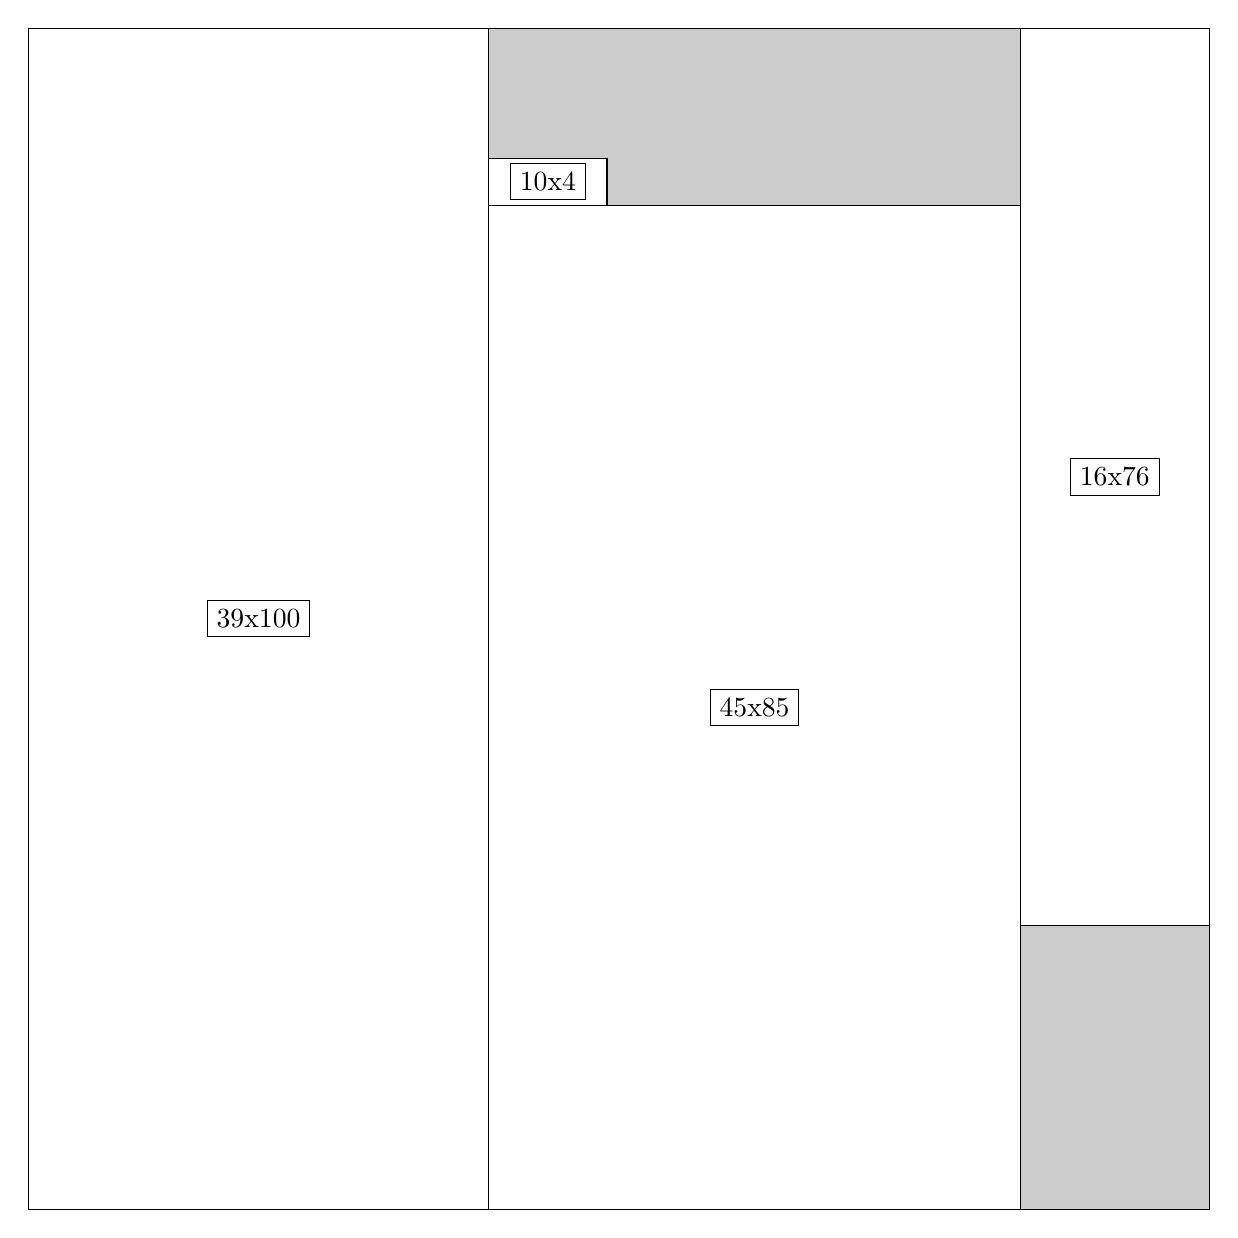
\begin{tikzpicture}[shorten >=1pt,scale=1.0,every node/.style={scale=1.0},->]
\tikzstyle{vertex}=[circle,fill=black!25,minimum size=14pt,inner sep=0pt]
\filldraw[fill=gray!40!white, draw=black] (0,0) rectangle (15.0,15.0);
\foreach \name/\x/\y/\w/\h in {39x100/0.0/0.0/5.85/15.0,45x85/5.85/0.0/6.75/12.75,16x76/12.6/3.5999999999999996/2.4/11.4,10x4/5.85/12.75/1.5/0.6}
\filldraw[fill=white!40!white, draw=black] (\x,\y) rectangle node[draw] (\name) {\name} ++(\w,\h);
\end{tikzpicture}


w =39 , h =100 , x =0 , y =0 , v =3900
\par
w =45 , h =85 , x =39 , y =0 , v =3825
\par
w =16 , h =76 , x =84 , y =24 , v =1216
\par
w =10 , h =4 , x =39 , y =85 , v =40
\par
\newpage


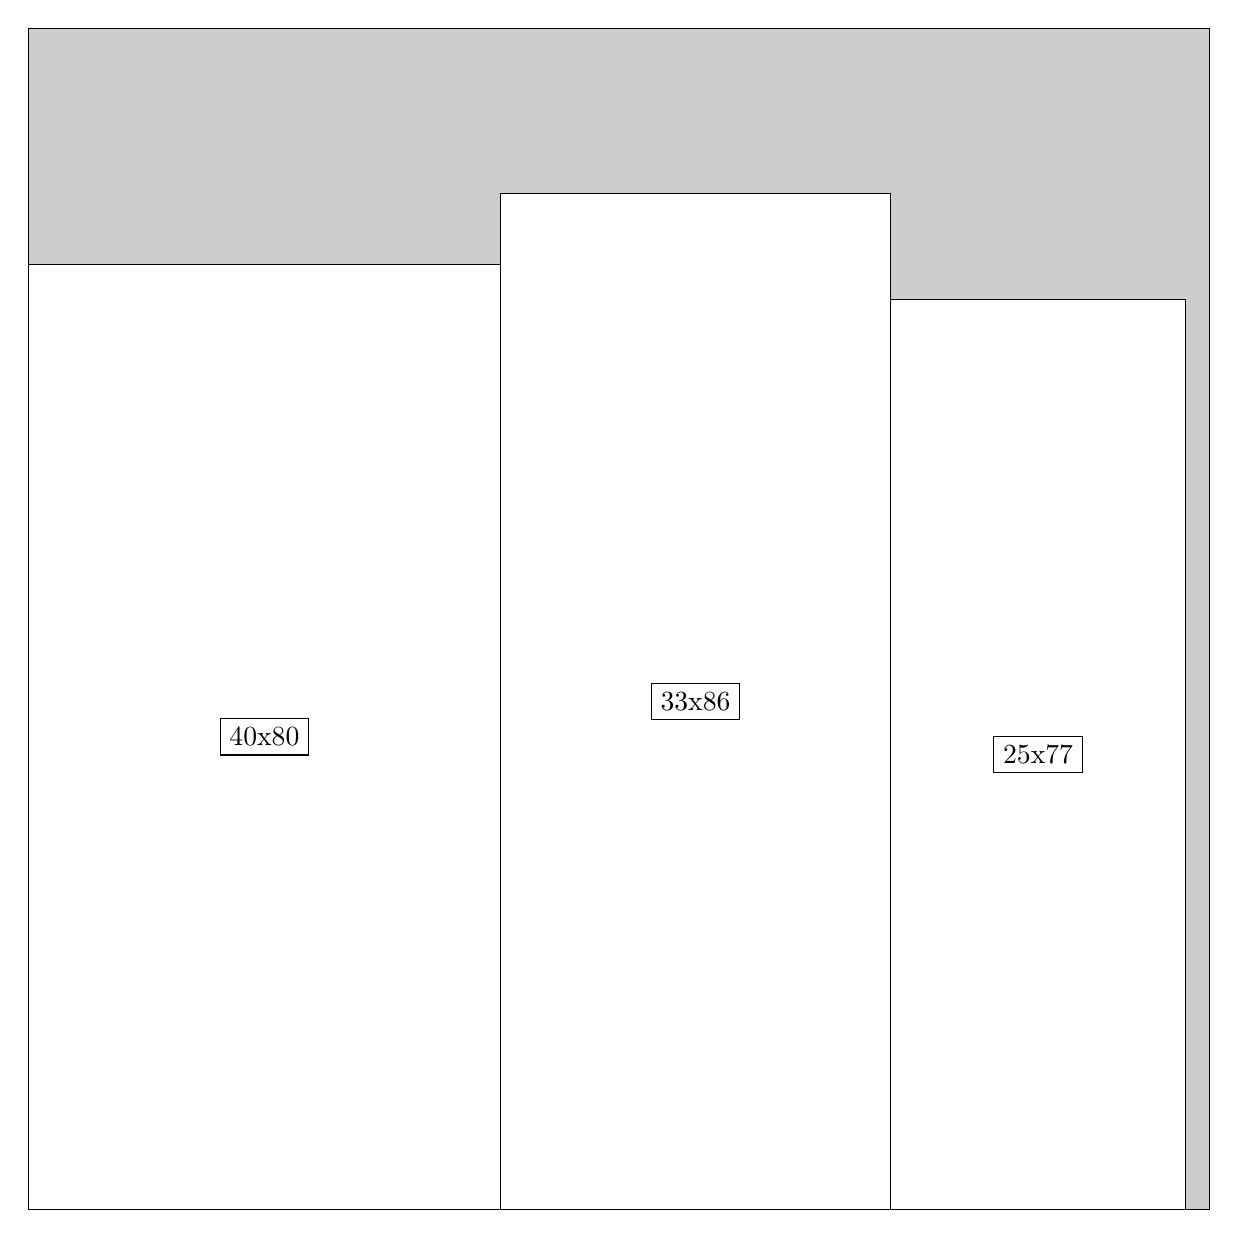
\begin{tikzpicture}[shorten >=1pt,scale=1.0,every node/.style={scale=1.0},->]
\tikzstyle{vertex}=[circle,fill=black!25,minimum size=14pt,inner sep=0pt]
\filldraw[fill=gray!40!white, draw=black] (0,0) rectangle (15.0,15.0);
\foreach \name/\x/\y/\w/\h in {40x80/0.0/0.0/6.0/12.0,33x86/6.0/0.0/4.95/12.9,25x77/10.95/0.0/3.75/11.549999999999999}
\filldraw[fill=white!40!white, draw=black] (\x,\y) rectangle node[draw] (\name) {\name} ++(\w,\h);
\end{tikzpicture}


w =40 , h =80 , x =0 , y =0 , v =3200
\par
w =33 , h =86 , x =40 , y =0 , v =2838
\par
w =25 , h =77 , x =73 , y =0 , v =1925
\par
\newpage


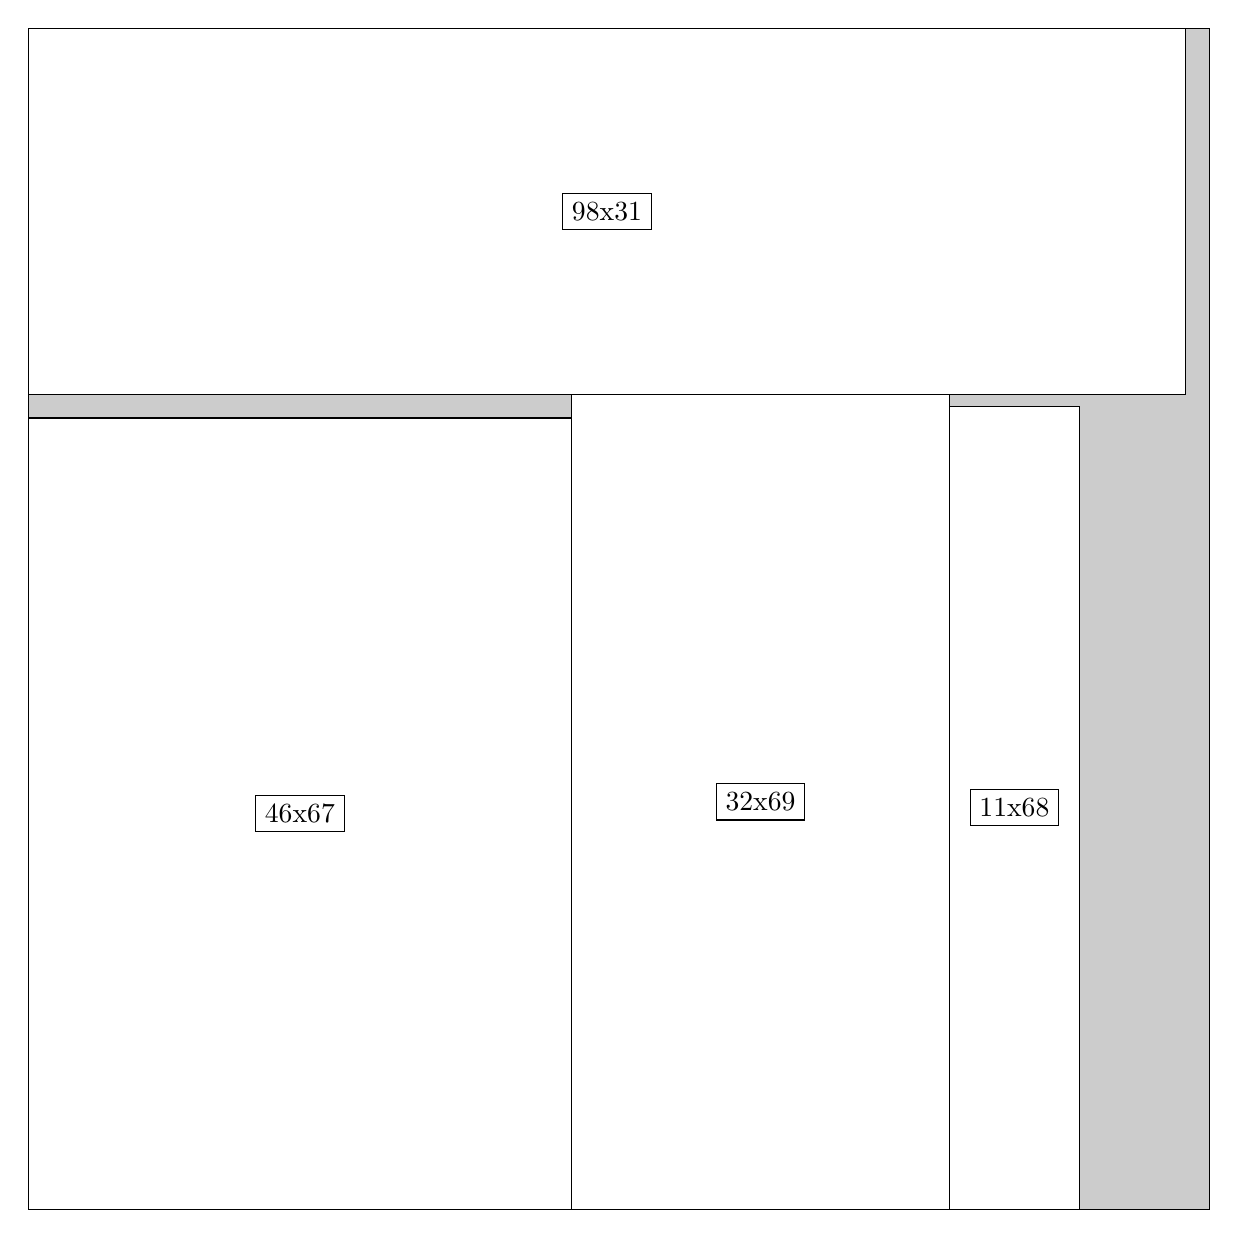
\begin{tikzpicture}[shorten >=1pt,scale=1.0,every node/.style={scale=1.0},->]
\tikzstyle{vertex}=[circle,fill=black!25,minimum size=14pt,inner sep=0pt]
\filldraw[fill=gray!40!white, draw=black] (0,0) rectangle (15.0,15.0);
\foreach \name/\x/\y/\w/\h in {46x67/0.0/0.0/6.8999999999999995/10.049999999999999,98x31/0.0/10.35/14.7/4.6499999999999995,32x69/6.8999999999999995/0.0/4.8/10.35,11x68/11.7/0.0/1.65/10.2}
\filldraw[fill=white!40!white, draw=black] (\x,\y) rectangle node[draw] (\name) {\name} ++(\w,\h);
\end{tikzpicture}


w =46 , h =67 , x =0 , y =0 , v =3082
\par
w =98 , h =31 , x =0 , y =69 , v =3038
\par
w =32 , h =69 , x =46 , y =0 , v =2208
\par
w =11 , h =68 , x =78 , y =0 , v =748
\par
\newpage


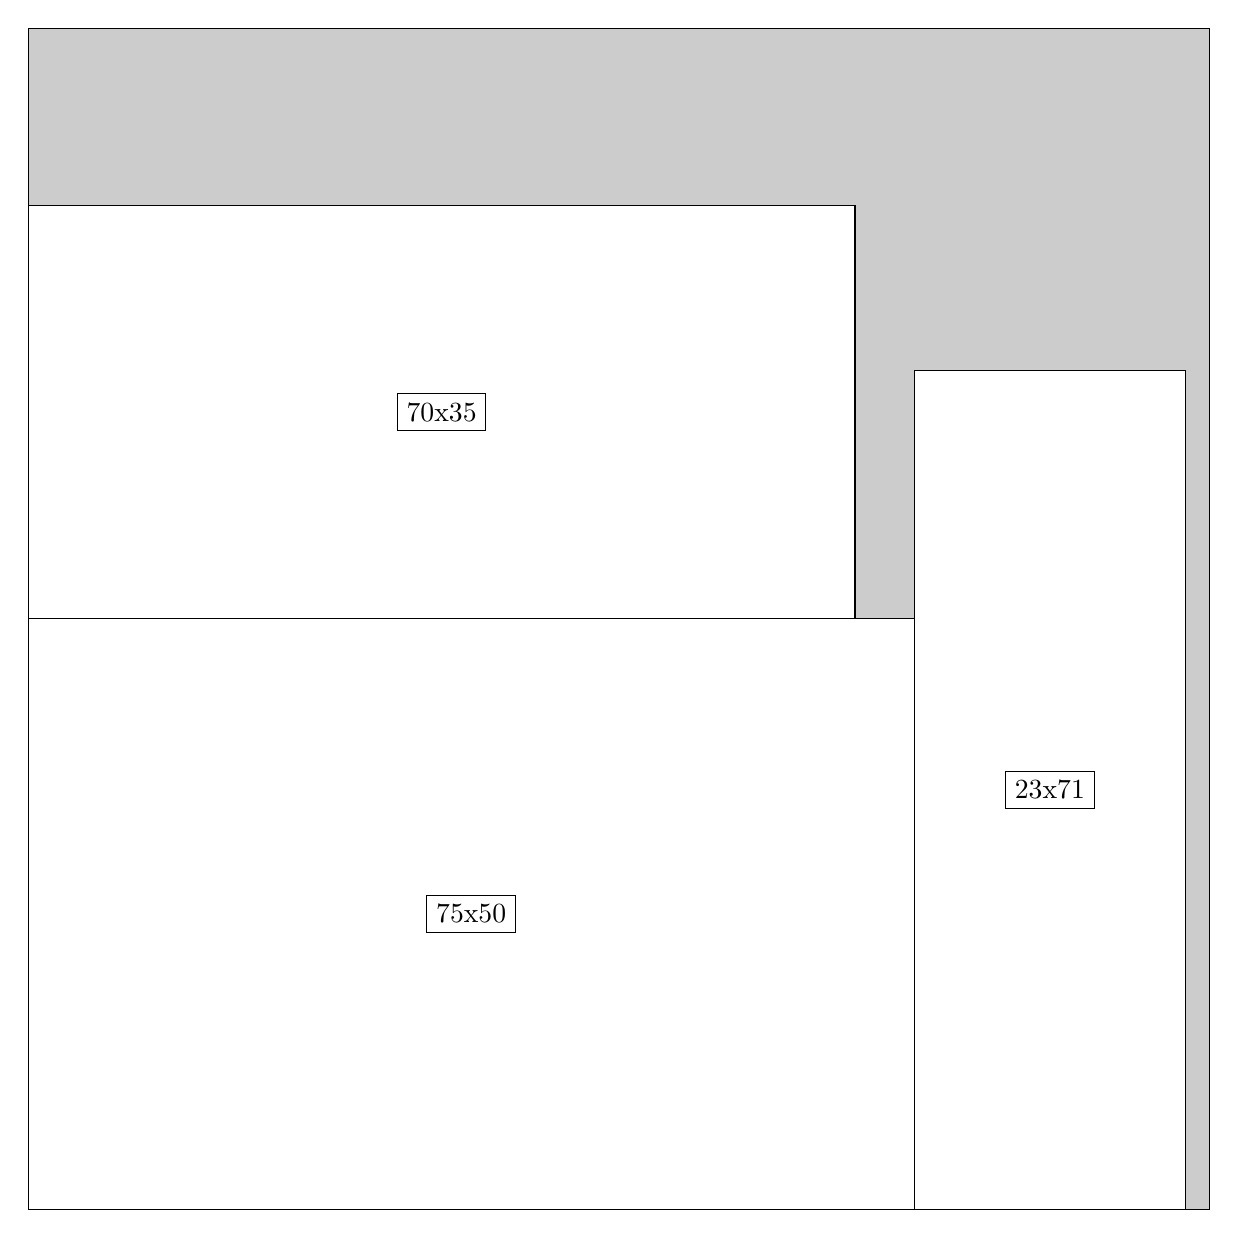
\begin{tikzpicture}[shorten >=1pt,scale=1.0,every node/.style={scale=1.0},->]
\tikzstyle{vertex}=[circle,fill=black!25,minimum size=14pt,inner sep=0pt]
\filldraw[fill=gray!40!white, draw=black] (0,0) rectangle (15.0,15.0);
\foreach \name/\x/\y/\w/\h in {75x50/0.0/0.0/11.25/7.5,70x35/0.0/7.5/10.5/5.25,23x71/11.25/0.0/3.4499999999999997/10.65}
\filldraw[fill=white!40!white, draw=black] (\x,\y) rectangle node[draw] (\name) {\name} ++(\w,\h);
\end{tikzpicture}


w =75 , h =50 , x =0 , y =0 , v =3750
\par
w =70 , h =35 , x =0 , y =50 , v =2450
\par
w =23 , h =71 , x =75 , y =0 , v =1633
\par
\newpage


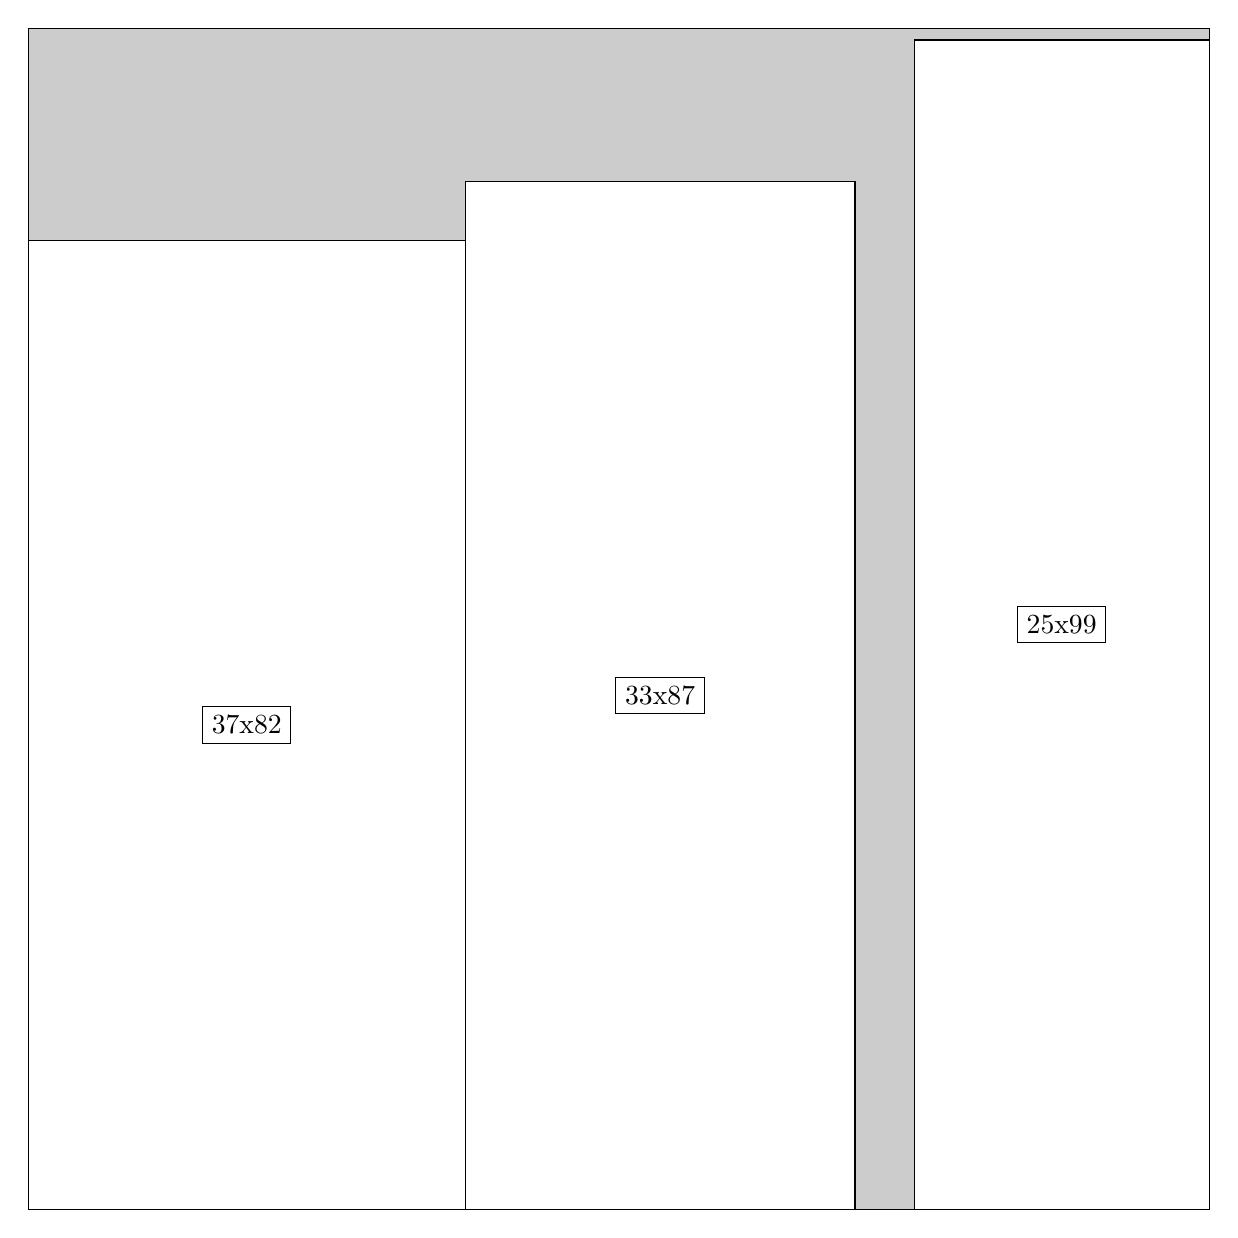
\begin{tikzpicture}[shorten >=1pt,scale=1.0,every node/.style={scale=1.0},->]
\tikzstyle{vertex}=[circle,fill=black!25,minimum size=14pt,inner sep=0pt]
\filldraw[fill=gray!40!white, draw=black] (0,0) rectangle (15.0,15.0);
\foreach \name/\x/\y/\w/\h in {37x82/0.0/0.0/5.55/12.299999999999999,33x87/5.55/0.0/4.95/13.049999999999999,25x99/11.25/0.0/3.75/14.85}
\filldraw[fill=white!40!white, draw=black] (\x,\y) rectangle node[draw] (\name) {\name} ++(\w,\h);
\end{tikzpicture}


w =37 , h =82 , x =0 , y =0 , v =3034
\par
w =33 , h =87 , x =37 , y =0 , v =2871
\par
w =25 , h =99 , x =75 , y =0 , v =2475
\par
\newpage


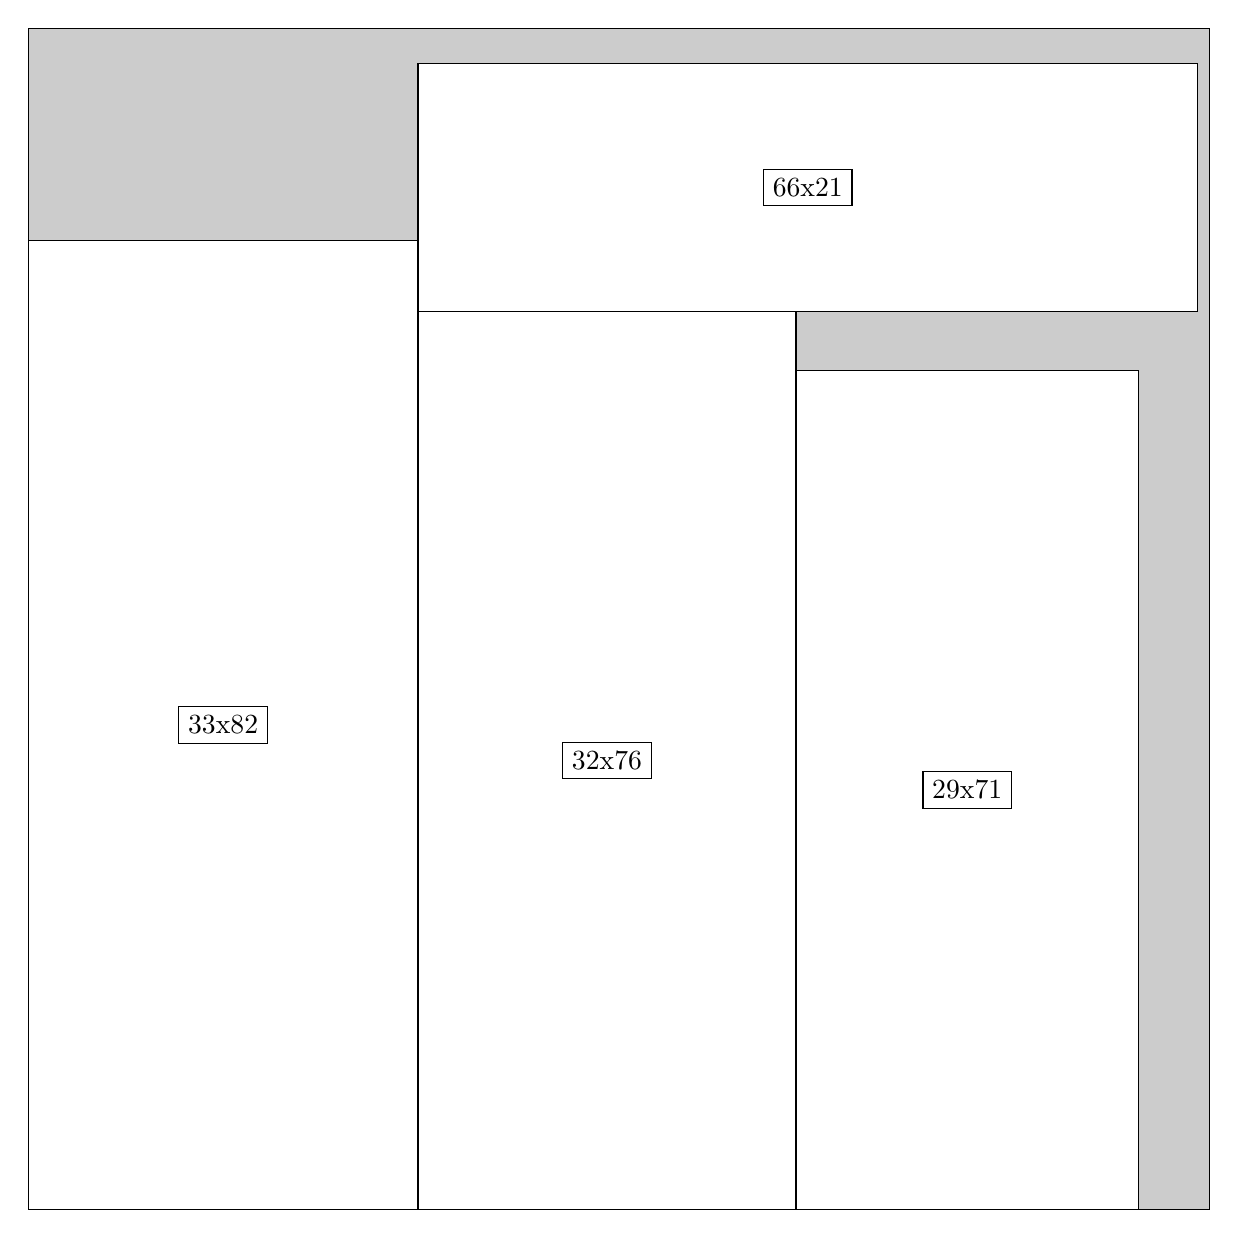
\begin{tikzpicture}[shorten >=1pt,scale=1.0,every node/.style={scale=1.0},->]
\tikzstyle{vertex}=[circle,fill=black!25,minimum size=14pt,inner sep=0pt]
\filldraw[fill=gray!40!white, draw=black] (0,0) rectangle (15.0,15.0);
\foreach \name/\x/\y/\w/\h in {33x82/0.0/0.0/4.95/12.299999999999999,32x76/4.95/0.0/4.8/11.4,29x71/9.75/0.0/4.35/10.65,66x21/4.95/11.4/9.9/3.15}
\filldraw[fill=white!40!white, draw=black] (\x,\y) rectangle node[draw] (\name) {\name} ++(\w,\h);
\end{tikzpicture}


w =33 , h =82 , x =0 , y =0 , v =2706
\par
w =32 , h =76 , x =33 , y =0 , v =2432
\par
w =29 , h =71 , x =65 , y =0 , v =2059
\par
w =66 , h =21 , x =33 , y =76 , v =1386
\par
\newpage


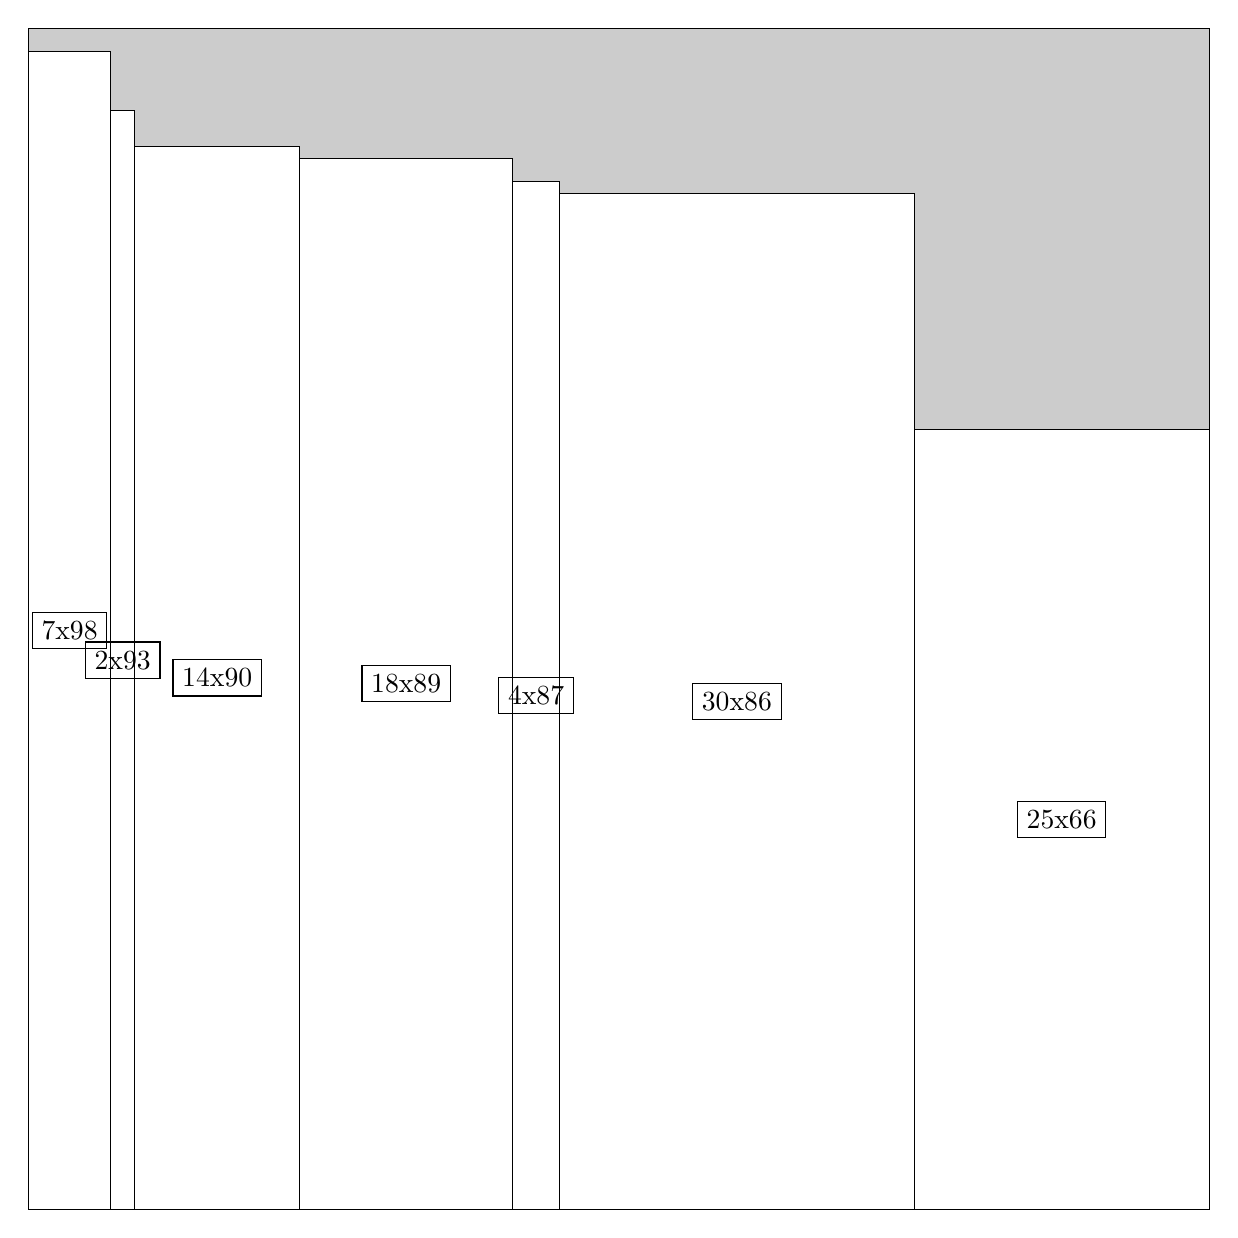
\begin{tikzpicture}[shorten >=1pt,scale=1.0,every node/.style={scale=1.0},->]
\tikzstyle{vertex}=[circle,fill=black!25,minimum size=14pt,inner sep=0pt]
\filldraw[fill=gray!40!white, draw=black] (0,0) rectangle (15.0,15.0);
\foreach \name/\x/\y/\w/\h in {30x86/6.75/0.0/4.5/12.9,25x66/11.25/0.0/3.75/9.9,18x89/3.4499999999999997/0.0/2.6999999999999997/13.35,14x90/1.3499999999999999/0.0/2.1/13.5,7x98/0.0/0.0/1.05/14.7,4x87/6.1499999999999995/0.0/0.6/13.049999999999999,2x93/1.05/0.0/0.3/13.95}
\filldraw[fill=white!40!white, draw=black] (\x,\y) rectangle node[draw] (\name) {\name} ++(\w,\h);
\end{tikzpicture}


w =30 , h =86 , x =45 , y =0 , v =2580
\par
w =25 , h =66 , x =75 , y =0 , v =1650
\par
w =18 , h =89 , x =23 , y =0 , v =1602
\par
w =14 , h =90 , x =9 , y =0 , v =1260
\par
w =7 , h =98 , x =0 , y =0 , v =686
\par
w =4 , h =87 , x =41 , y =0 , v =348
\par
w =2 , h =93 , x =7 , y =0 , v =186
\par
\newpage


\end{document}